% notes.tex

See \cite{AbbottUnderstandingAnalysis} for an intuition-driven introduction
to upper and lower bounds and the least upper bound property.

% =========================================================
% Field Axioms of the Real Numbers
% =========================================================

\subsection{Field Axioms of the Real Numbers}

The real numbers $\mathbb{R}$ form a \emph{field}. This means that $\mathbb{R}$ is a set
equipped with two binary operations, addition $(+)$ and multiplication $(\cdot)$,
satisfying the following axioms.

\subsubsection*{Additive Axioms}

\begin{description}

\item[\textbf{Axiom A1 (Additive Closure).}]
For all $x,y \in \mathbb{R}$, the sum $x+y \in \mathbb{R}$.
\[
\forall x \forall y \, (x,y \in \mathbb{R} \rightarrow x+y \in \mathbb{R})
\]

\item[\textbf{Axiom A2 (Additive Commutativity).}]
For all $x,y \in \mathbb{R}$,
\[
x+y = y+x.
\]
\[
\forall x \forall y \, (x+y = y+x)
\]

\item[\textbf{Axiom A3 (Additive Associativity).}]
For all $x,y,z \in \mathbb{R}$,
\[
(x+y)+z = x+(y+z).
\]
\[
\forall x \forall y \forall z \, ((x+y)+z = x+(y+z))
\]

\item[\textbf{Axiom A4 (Additive Identity).}]
There exists an element $0 \in \mathbb{R}$ such that for all $x \in \mathbb{R}$,
\[
x+0 = x.
\]
\[
\exists 0 \, \forall x \, (x+0 = x)
\]

\item[\textbf{Axiom A5 (Additive Inverse).}]
For every $x \in \mathbb{R}$, there exists an element $-x \in \mathbb{R}$ such that
\[
x+(-x) = 0.
\]
\[
\forall x \, \exists y \, (x+y = 0)
\]

\end{description}

\subsubsection*{Multiplicative Axioms}

\begin{description}

\item[\textbf{Axiom M1 (Multiplicative Closure).}]
For all $x,y \in \mathbb{R}$, the product $x\cdot y \in \mathbb{R}$.
\[
\forall x \forall y \, (x,y \in \mathbb{R} \rightarrow x\cdot y \in \mathbb{R})
\]

\item[\textbf{Axiom M2 (Multiplicative Commutativity).}]
For all $x,y \in \mathbb{R}$,
\[
x\cdot y = y\cdot x.
\]
\[
\forall x \forall y \, (x\cdot y = y\cdot x)
\]

\item[\textbf{Axiom M3 (Multiplicative Associativity).}]
For all $x,y,z \in \mathbb{R}$,
\[
(x\cdot y)\cdot z = x\cdot (y\cdot z).
\]
\[
\forall x \forall y \forall z \, ((x\cdot y)\cdot z = x\cdot (y\cdot z))
\]

\item[\textbf{Axiom M4 (Multiplicative Identity).}]
There exists an element $1 \in \mathbb{R}$, with $1 \neq 0$, such that for all $x \in \mathbb{R}$,
\[
x\cdot 1 = x.
\]
\[
\exists 1 \, (1 \neq 0 \wedge \forall x \, (x\cdot 1 = x))
\]

\item[\textbf{Axiom M5 (Multiplicative Inverse).}]
For every $x \in \mathbb{R}$ with $x \neq 0$, there exists an element $x^{-1} \in \mathbb{R}$ such that
\[
x\cdot x^{-1} = 1.
\]
\[
\forall x \, (x \neq 0 \rightarrow \exists y \, (x\cdot y = 1))
\]

\end{description}

\subsubsection*{Distributive Axiom}

\begin{description}

\item[\textbf{Axiom D (Distributivity).}]
For all $x,y,z \in \mathbb{R}$,
\[
x\cdot (y+z) = x\cdot y + x\cdot z.
\]
\[
\forall x \forall y \forall z \, (x\cdot (y+z) = x\cdot y + x\cdot z)
\]

\end{description}

\subsubsection*{Remark}

The axioms above define the algebraic structure of a field. To characterize
$\mathbb{R}$ uniquely among fields, these axioms must be supplemented by:
\begin{itemize}
\item an \emph{order structure} (ordered field axioms), and
\item the \emph{completeness axiom}.
\end{itemize}



% =========================================================
% Order Axioms of the Real Numbers
% =========================================================

\subsection{Order Axioms of the Real Numbers}


The real numbers $\mathbb{R}$ form a \emph{totally ordered field}.
The order structure is given by a binary relation $\le$ on $\mathbb{R}$
satisfying the following axioms.

% ---------------------------------------------------------
% Linear (Total) Order
% ---------------------------------------------------------

\subsubsection*{Linear Order Axioms}

\begin{description}

\item[\textbf{O1 (Reflexivity).}]
\[
\forall x\in\mathbb{R},\quad x \le x.
\]

\item[\textbf{O2 (Antisymmetry).}]
\[
\forall x,y\in\mathbb{R},\quad
(x \le y \wedge y \le x) \rightarrow x = y.
\]

\item[\textbf{O3 (Transitivity).}]
\[
\forall x,y,z\in\mathbb{R},\quad
(x \le y \wedge y \le z) \rightarrow x \le z.
\]

\item[\textbf{O4 (Totality / Comparability).}]
\[
\forall x,y\in\mathbb{R},\quad
x \le y \ \vee\ y \le x.
\]

\end{description}

\medskip

These axioms state that $(\mathbb{R},\le)$ is a \emph{linear (total) order}.
The strict order $<$ is defined by
\[
x < y \quad\text{if and only if}\quad x \le y \text{ and } x \neq y.
\]

% ---------------------------------------------------------
% Compatibility with Field Operations
% ---------------------------------------------------------

\subsubsection*{Order Compatibility with Field Operations}

\begin{description}

\item[\textbf{O5 (Additive Monotonicity).}]
\[
\forall x,y,z\in\mathbb{R},\quad
x \le y \rightarrow x+z \le y+z.
\]

\item[\textbf{O6 (Multiplicative Monotonicity for Nonnegative Factors).}]
\[
\forall x,y,z\in\mathbb{R},\quad
(x \le y \wedge 0 \le z) \rightarrow xz \le yz.
\]

\item[\textbf{O7 (Positivity of the Unit).}]
\[
0 < 1.
\]

\end{description}

\subsubsection*{Remark}

Axiom \textup{O6} implies that multiplication by a negative number reverses
inequalities; this fact will be proved later as a theorem and is not taken
as a separate axiom.

Together with the field axioms, these order axioms make $\mathbb{R}$
an \emph{ordered field}. To characterize $\mathbb{R}$ uniquely among ordered
fields, one must additionally assume the \emph{completeness axiom}.



% =========================================================
% Intervals
% =========================================================

\subsection{Intervals in the Real Numbers}

Intervals are fundamental subsets of the real line defined using the order
relation on $\mathbb{R}$. Let $a,b \in \mathbb{R}$ with $a < b$.

\subsubsection*{Bounded Intervals}

\begin{definition}[Open Interval]
The \emph{open interval} from $a$ to $b$ is the set
\[
(a,b) := \{ x \in \mathbb{R} : a < x < b \}.
\]
\[
\forall x \, (x \in (a,b) \leftrightarrow a < x \wedge x < b)
\]
\end{definition}

\begin{definition}[Closed Interval]
The \emph{closed interval} from $a$ to $b$ is the set
\[
[a,b] := \{ x \in \mathbb{R} : a \le x \le b \}.
\]
\[
\forall x \, (x \in [a,b] \leftrightarrow a \le x \wedge x \le b)
\]
\end{definition}

\begin{definition}[Half-Open Intervals]
The \emph{left-closed, right-open interval} is
\[
[a,b) := \{ x \in \mathbb{R} : a \le x < b \}.
\]
The \emph{left-open, right-closed interval} is
\[
(a,b] := \{ x \in \mathbb{R} : a < x \le b \}.
\]
\end{definition}

\subsubsection*{Unbounded Intervals}

\begin{definition}[Open Rays]
The \emph{open rays} determined by $a \in \mathbb{R}$ are
\[
(a,\infty) := \{ x \in \mathbb{R} : x > a \},
\qquad
(-\infty,a) := \{ x \in \mathbb{R} : x < a \}.
\]
\end{definition}

\begin{definition}[Closed Rays]
The \emph{closed rays} determined by $a \in \mathbb{R}$ are
\[
[a,\infty) := \{ x \in \mathbb{R} : x \ge a \},
\qquad
(-\infty,a] := \{ x \in \mathbb{R} : x \le a \}.
\]
\end{definition}

\subsubsection*{Degenerate and Trivial Intervals}

\begin{definition}[Degenerate Interval]
If $a=b$, the closed interval
\[
[a,a] = \{a\}
\]
is called a \emph{degenerate interval}.
\end{definition}

\begin{definition}[Empty Interval]
If $a>b$, the set
\[
(a,b) = \varnothing
\]
is called an \emph{empty interval}.
\end{definition}

\begin{remark}
Intervals are precisely the subsets of $\mathbb{R}$ with the property that if
$x<y<z$ and $x,z$ belong to the set, then $y$ also belongs to the set.
\end{remark}



% =========================================================
% Bounds, Suprema, Infima + Table + Figure
% =========================================================

\subsection{Bounds and Extremal Values}

\begin{figure}[h]
\centering
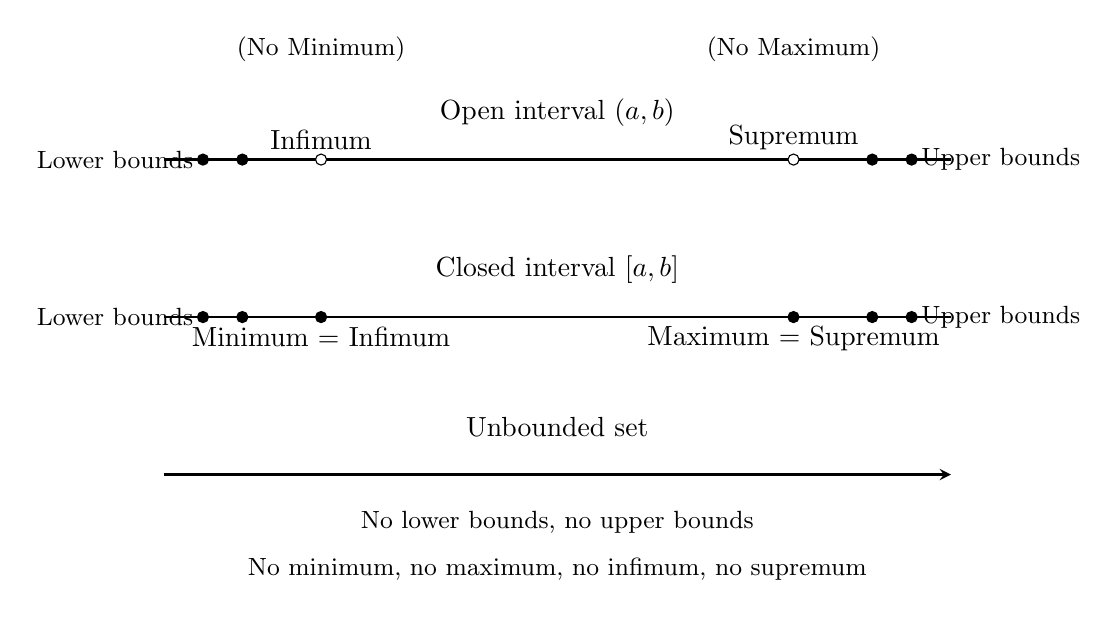
\begin{tikzpicture}[x=1cm,y=1cm,>=stealth]

% =====================
% OPEN INTERVAL (a,b)
% =====================
\draw[thick] (-5,3) -- (5,3);
\draw[fill=white] (-3,3) circle (2pt);
\draw[fill=white] (3,3) circle (2pt);

\node at (0,3.6) {Open interval $(a,b)$};

% Infimum / Supremum
\node[above] at (-3,3) {Infimum};
\node[above] at (3,3) {Supremum};
\node at (-3,4.4) {\small (No Minimum)};
\node at (3,4.4) {\small (No Maximum)};

% Lower bounds
\draw[fill] (-4.5,3) circle (2pt);
\draw[fill] (-4,3) circle (2pt);
\node[left] at (-4.5,3) {\small Lower bounds};

% Upper bounds
\draw[fill] (4,3) circle (2pt);
\draw[fill] (4.5,3) circle (2pt);
\node[right] at (4.5,3) {\small Upper bounds};

% =====================
% CLOSED INTERVAL [a,b]
% =====================
\draw[thick] (-5,1) -- (5,1);
\draw[fill] (-3,1) circle (2pt);
\draw[fill] (3,1) circle (2pt);

\node at (0,1.6) {Closed interval $[a,b]$};

% Min / Max
\node[below] at (-3,1) {Minimum = Infimum};
\node[below] at (3,1) {Maximum = Supremum};

% Lower bounds
\draw[fill] (-4.5,1) circle (2pt);
\draw[fill] (-4,1) circle (2pt);
\node[left] at (-4.5,1) {\small Lower bounds};

% Upper bounds
\draw[fill] (4,1) circle (2pt);
\draw[fill] (4.5,1) circle (2pt);
\node[right] at (4.5,1) {\small Upper bounds};

% =====================
% UNBOUNDED SET
% =====================
\draw[thick,->] (-5,-1) -- (5,-1);

\node at (0,-0.4) {Unbounded set};

\node at (0,-1.6)
{\small No lower bounds, no upper bounds};

\node at (0,-2.2)
{\small No minimum, no maximum, no infimum, no supremum};

\end{tikzpicture}
\caption{Bounds, extrema, infimum, and supremum for subsets of $\mathbb{R}$.}
\end{figure}

\begin{center}
\begin{tabular}{|p{4cm}|p{9cm}|}
\hline
\textbf{Concept} & \textbf{What you must show} \\
\hline

Upper bound &
To show that $u$ is an upper bound for $A$, prove that
\[
\forall a \in A,\quad a \le u.
\]
\\ \hline

Supremum &
To show that $u=\sup A$, prove:
\begin{itemize}
\item $u$ is an upper bound for $A$, and
\item every upper bound $v$ of $A$ satisfies $u \le v$.
\end{itemize}
\\ \hline

Bounded above &
To show that $A$ is bounded above, prove that
there exists at least one upper bound for $A$.
\\ \hline

Maximum &
To show that $m=\max A$, prove that $m$ is an upper bound for $A$
and that $m \in A$.
\\ \hline

\end{tabular}
\end{center}

\begin{definition}[Upper Bound]
Let $A \subseteq \mathbb{R}$.
A number $u \in \mathbb{R}$ is an \emph{upper bound} for $A$ if
\[
\forall a \in A,\quad a \le u.
\]
\end{definition}

\begin{definition}[Lower Bound]
Let $A \subseteq \mathbb{R}$.
A number $\ell \in \mathbb{R}$ is a \emph{lower bound} for $A$ if
\[
\forall a \in A,\quad \ell \le a.
\]
\end{definition}

\begin{definition}[Bounded Above / Below]
A set $A \subseteq \mathbb{R}$ is said to be:
\begin{itemize}
\item \emph{bounded above} if it has at least one upper bound;
\item \emph{bounded below} if it has at least one lower bound;
\item \emph{bounded} if it is both bounded above and bounded below.
\end{itemize}
\end{definition}

\begin{definition}[Supremum (Least Upper Bound)]
Let $A \subseteq \mathbb{R}$ be nonempty and bounded above.
A number $s \in \mathbb{R}$ is the \emph{supremum} of $A$, written $s=\sup A$, if:
\begin{enumerate}
\item $s$ is an upper bound for $A$, and
\item if $u$ is any upper bound for $A$, then $s \le u$.
\end{enumerate}
\end{definition}

\begin{definition}[Infimum (Greatest Lower Bound)]
Let $A \subseteq \mathbb{R}$ be nonempty and bounded below.
A number $i \in \mathbb{R}$ is the \emph{infimum} of $A$, written $i=\inf A$, if:
\begin{enumerate}
\item $i$ is a lower bound for $A$, and
\item if $\ell$ is any lower bound for $A$, then $\ell \le i$.
\end{enumerate}
\end{definition}

\begin{definition}[Maximum]
Let $A \subseteq \mathbb{R}$.
A number $m \in A$ is a \emph{maximum} of $A$, written $m=\max A$, if
\[
\forall a \in A,\quad a \le m.
\]
\end{definition}

\begin{definition}[Minimum]
Let $A \subseteq \mathbb{R}$.
A number $m \in A$ is a \emph{minimum} of $A$, written $m=\min A$, if
\[
\forall a \in A,\quad m \le a.
\]
\end{definition}

\subsubsection{Epsilon Characterizations}

\begin{definition}[Supremum — $\varepsilon$ Definition]
Let $A \subseteq \mathbb{R}$ be nonempty and bounded above, and let $s \in \mathbb{R}$.
Then $s = \sup A$ if and only if:
\begin{enumerate}
\item $s$ is an upper bound for $A$, and
\item for every $\varepsilon > 0$, there exists $a \in A$ such that
\[
s - \varepsilon < a.
\]
\end{enumerate}
\end{definition}

\begin{definition}[Infimum — $\varepsilon$ Definition]
Let $A \subseteq \mathbb{R}$ be nonempty and bounded below, and let $i \in \mathbb{R}$.
Then $i = \inf A$ if and only if:
\begin{enumerate}
\item $i$ is a lower bound for $A$, and
\item for every $\varepsilon > 0$, there exists $a \in A$ such that
\[
a < i + \varepsilon.
\]
\end{enumerate}
\end{definition}

\subsubsection{Directional $\varepsilon$-Characterizations}

\paragraph{Supremum: $\varepsilon$-approximation from below}
If $s=\sup A$, then
\[
\forall \varepsilon>0,\ \exists a\in A \ \text{such that}\ s-\varepsilon < a \le s.
\]

\paragraph{Infimum: $\varepsilon$-approximation from above}
If $i=\inf A$, then
\[
\forall \varepsilon>0,\ \exists a\in A \ \text{such that}\ i \le a < i+\varepsilon.
\]

\medskip

See \cite{RossElementaryAnalysis} for a clean axiomatic development of
bounds, suprema, and infima within ordered fields.

See \cite{BrucknerRealAnalysis} for a technically precise treatment of
bounds and extrema, including early exposure to subtle and pathological
examples.

See \cite{KolmogorovFominIntroAnalysis} for a classical, structurally
oriented approach to bounds and completeness with minimal pedagogical
scaffolding.

See \cite{LeblBasicAnalysisI} for a modern exposition of bounds and the
least upper bound property, accompanied by an extensive and well-curated
problem set.



% =========================================================
% Completeness Axiom (Short)
% =========================================================

\subsection{Axiom of Completeness}

\begin{axiom}[Completeness Axiom (Least Upper Bound Property)]
Every nonempty subset of $\mathbb{R}$ that is bounded above has a supremum in $\mathbb{R}$.
Equivalently, if $S\subseteq\mathbb{R}$ is nonempty and bounded above, then $\sup S$ exists
as a real number.
\end{axiom}

\begin{remark}[Logical form]
\[
\forall S\;\Bigl(
(S\subseteq\mathbb{R}\wedge S\neq\varnothing\wedge \exists M\in\mathbb{R}\ \forall x\in S\ (x\le M))
\rightarrow
\exists s\in\mathbb{R}\ (s=\sup S)
\Bigr).
\]
\end{remark}

\begin{remark}[Common equivalent formulations]
The completeness axiom is equivalent (over the ordered-field axioms) to each of the following:
\begin{itemize}
\item Every nonempty set bounded below has an infimum.
\item Every Cauchy sequence in $\mathbb{R}$ converges in $\mathbb{R}$.
\item (Nested interval property) Every nested sequence of nonempty closed intervals with lengths $\to 0$
has nonempty intersection.
\end{itemize}
\end{remark}

% =========================================================
% Nested Interval Property (Theorem + Proof)
% =========================================================

\begin{theorem}[Nested Interval Property]
Let $\{[a_n,b_n]\}_{n\in\mathbb{N}}$ be a sequence of nonempty closed intervals in $\mathbb{R}$
such that
\[
[a_{n+1},b_{n+1}] \subseteq [a_n,b_n]
\quad\text{for all } n\in\mathbb{N}.
\]
Then
\[
\bigcap_{n=1}^\infty [a_n,b_n] \neq \varnothing.
\]
Moreover, if in addition $b_n-a_n \to 0$, then the intersection consists of exactly one point.
\end{theorem}

\begin{proof}
Because $[a_{n+1},b_{n+1}] \subseteq [a_n,b_n]$, we have
\[
a_n \le a_{n+1}
\quad\text{and}\quad
b_{n+1} \le b_n
\quad\text{for all } n.
\]
In particular, for each $n$ we have $a_n \le b_n$, so $\{a_n\}$ is bounded above by (for example) $b_1$.

By completeness, the set $\{a_n : n\in\mathbb{N}\}$ has a supremum. Define
\[
a := \sup\{a_n : n\in\mathbb{N}\}.
\]

\medskip
\noindent\emph{Claim: $a \in [a_n,b_n]$ for every $n$.}

\smallskip
\noindent First, since $a$ is an upper bound for $\{a_n\}$, we have
\[
a_n \le a
\quad\text{for all } n.
\]

\smallskip
\noindent Next, fix $n$. For every $k\ge n$ we have $a_k \in [a_k,b_k]\subseteq [a_n,b_n]$, hence
\[
a_k \le b_n
\quad\text{for all } k\ge n.
\]
Therefore $b_n$ is an upper bound for the tail set $\{a_k : k\ge n\}$, so
\[
a = \sup\{a_k : k\in\mathbb{N}\} \le b_n.
\]
Combining, $a_n \le a \le b_n$, i.e.\ $a\in [a_n,b_n]$.

\medskip
Thus $a\in \bigcap_{n=1}^\infty [a_n,b_n]$, proving the intersection is nonempty.

\medskip
\noindent\emph{Uniqueness when $b_n-a_n\to 0$.}
If $x,y \in \bigcap_{n=1}^\infty [a_n,b_n]$, then for every $n$,
\[
a_n \le x \le b_n
\quad\text{and}\quad
a_n \le y \le b_n,
\]
so $|x-y| \le b_n-a_n$. Taking $n\to\infty$ and using $b_n-a_n\to 0$ gives $|x-y|=0$, hence $x=y$.
Therefore the intersection contains exactly one point.
\end{proof}


% =========================================================
% Archimedean, Floor Lemma, Density of Q, Square Roots
% =========================================================

\subsection{Other Properties of the Real Numbers}

\begin{definition}[Archimedean Property]
The real numbers $\mathbb{R}$ are said to satisfy the \emph{Archimedean property} if
\[
\forall x \in \mathbb{R}\;\exists n \in \mathbb{N}\;\; (n > x).
\]
Equivalently, for all $x>0$ and all $y\in\mathbb{R}$ there exists $n\in\mathbb{N}$ such that
\[
nx > y.
\]
\end{definition}

\begin{remark}[Logical form]
\[
\forall x\,\Bigl(x\in\mathbb{R}\rightarrow \exists n\,\bigl(n\in\mathbb{N}\wedge n>x\bigr)\Bigr).
\]
\[
\forall x\,\forall y\,\Bigl((x\in\mathbb{R}\wedge y\in\mathbb{R}\wedge x>0)\rightarrow
\exists n\,\bigl(n\in\mathbb{N}\wedge nx>y\bigr)\Bigr).
\]
\end{remark}

\begin{theorem}[Archimedean Property of $\mathbb{R}$]
The real numbers $\mathbb{R}$ satisfy the Archimedean property.
\end{theorem}

\begin{proof}
Assume for contradiction that the Archimedean property fails. Then there exists
$x\in\mathbb{R}$ such that
\[
\forall n\in\mathbb{N},\quad n \le x.
\]
Thus $\mathbb{N}$ is bounded above, so by completeness $\sup\mathbb{N}$ exists in $\mathbb{R}$.
Let $s := \sup \mathbb{N}$.

Then $s-1$ cannot be an upper bound of $\mathbb{N}$, hence there exists $m\in\mathbb{N}$ such that
$m > s-1$. Adding $1$ yields $m+1 > s$, contradicting that $s$ is an upper bound of $\mathbb{N}$.
\end{proof}

\begin{corollary}[Scaled Archimedean form]
If $x>0$ and $y\in\mathbb{R}$, then $\exists n\in\mathbb{N}$ such that $nx>y$.
\end{corollary}

\begin{proof}
Apply the Archimedean property to $y/x\in\mathbb{R}$ to obtain $n\in\mathbb{N}$ with $n>y/x$,
then multiply by $x>0$.
\end{proof}

\begin{lemma}[Integer part / floor lemma]
For every $x\in\mathbb{R}$ there exists an integer $m\in\mathbb{Z}$ such that
\[
m \le x < m+1.
\]
\end{lemma}

\begin{definition}[Density]
Let $(X,<)$ be a linearly ordered set and let $A\subseteq X$.
We say that $A$ is \emph{dense in $X$} if
\[
\forall a,b\in X\;\bigl(a<b \rightarrow \exists c\in A\;(a<c<b)\bigr).
\]
\end{definition}

\begin{remark}[Logical form for $\mathbb{Q}$ dense in $\mathbb{R}$]
\[
\forall a\,\forall b\;\Bigl(\bigl(a\in\mathbb{R}\wedge b\in\mathbb{R}\wedge a<b\bigr)
\rightarrow \exists q\;\bigl(q\in\mathbb{Q}\wedge a<q<b\bigr)\Bigr).
\]
\end{remark}

\begin{theorem}[Density of $\mathbb{Q}$ in $\mathbb{R}$]
The rationals $\mathbb{Q}$ are dense in $\mathbb{R}$.
\end{theorem}

\begin{proof}
Let $a,b\in\mathbb{R}$ with $a<b$. Set $\varepsilon := b-a>0$.
By the Archimedean property, choose $n\in\mathbb{N}$ such that
\[
\frac{1}{n} < \varepsilon.
\]
Consider $x := na \in \mathbb{R}$. By the floor lemma, choose $m\in\mathbb{Z}$ such that
\[
m \le na < m+1.
\]
Define
\[
q := \frac{m+1}{n}\in\mathbb{Q}.
\]
Then $na < m+1$, so dividing by $n>0$ gives $a<q$.
Also, from $m \le na$ we get $m+1 \le na+1$, hence
\[
q=\frac{m+1}{n} \le a+\frac{1}{n} < a+(b-a)=b.
\]
Thus $a<q<b$.
\end{proof}

\begin{corollary}[Between any two rationals lies an irrational]
For all $r,s\in\mathbb{Q}$ with $r<s$, there exists $\alpha\in\mathbb{R}\setminus\mathbb{Q}$ such that
\[
r<\alpha<s.
\]
\end{corollary}

\begin{proof}
Let $r,s\in\mathbb{Q}$ with $r<s$ and set $\varepsilon:=s-r>0$.
Choose $n\in\mathbb{N}$ such that
\[
\frac{\sqrt{2}}{n} < \varepsilon.
\]
Define
\[
\alpha := r + \frac{\sqrt{2}}{n}.
\]
Then $r<\alpha<s$.

If $\alpha\in\mathbb{Q}$ then $\alpha-r\in\mathbb{Q}$, hence $\sqrt{2}/n\in\mathbb{Q}$, so
$\sqrt{2}\in\mathbb{Q}$, a contradiction. Therefore $\alpha\notin\mathbb{Q}$.
\end{proof}

\begin{corollary}[Density of irrationals in $\mathbb{R}$]
The set $\mathbb{R}\setminus\mathbb{Q}$ is dense in $\mathbb{R}$; i.e.,
\[
\forall a,b\in\mathbb{R}\;\bigl(a<b \rightarrow \exists \alpha\in\mathbb{R}\setminus\mathbb{Q}\;(a<\alpha<b)\bigr).
\]
\end{corollary}

\begin{proof}
Let $a<b$ in $\mathbb{R}$. By density of $\mathbb{Q}$ choose $r,s\in\mathbb{Q}$ with $a<r<s<b$.
By the previous corollary choose $\alpha\in\mathbb{R}\setminus\mathbb{Q}$ with $r<\alpha<s$.
Then $a<\alpha<b$.
\end{proof}

\begin{theorem}[Existence of square roots]
For every real number $a \ge 0$, there exists a unique real number $x \ge 0$ such that
\[
x^2 = a.
\]
This number is denoted by $\sqrt{a}$.
\end{theorem}

\begin{remark}[Logical form]
\[
\forall a\;\Bigl(\bigl(a\in\mathbb{R}\wedge a\ge 0\bigr)
\rightarrow \exists!\,x\;\bigl(x\in\mathbb{R}\wedge x\ge 0 \wedge x^2=a\bigr)\Bigr).
\]
\end{remark}

\begin{proof}[Existence]
Fix $a\ge 0$. If $a=0$, take $x=0$. Assume $a>0$ and define
\[
S := \{x\in\mathbb{R} : x\ge 0 \text{ and } x^2 \le a\}.
\]
Then $S$ is nonempty and bounded above. By completeness, $s:=\sup S$ exists.

We show $s^2=a$.

\medskip
\noindent\emph{Claim 1: $s^2\le a$.}
If $s^2>a$, choose $\varepsilon>0$ such that $(s-\varepsilon)^2>a$. Then $s-\varepsilon$ is
still an upper bound for $S$, contradicting minimality of $s$.

\medskip
\noindent\emph{Claim 2: $s^2\ge a$.}
If $s^2<a$, let
\[
\delta := \min\left\{1,\frac{a-s^2}{2s+1}\right\}>0.
\]
Then
\[
(s+\delta)^2 = s^2 + 2s\delta + \delta^2 \le s^2 + (2s+1)\delta \le a,
\]
so $s+\delta\in S$, contradicting that $s$ is an upper bound.

Therefore $s^2=a$ and $s\ge 0$.
\end{proof}

\begin{proof}[Uniqueness]
Suppose $x,y\ge 0$ and $x^2=y^2$. Then
\[
(x-y)(x+y)=0.
\]
Since $x+y>0$, it follows that $x=y$.
\end{proof}



% =========================================================
% Metric Space / Modulus / Metrics (Vertical Layout)
% =========================================================

\subsection{Real Numbers as a Metric Space}

\begin{definition}[Modulus / Absolute value]
The \emph{modulus} (absolute value) is the function
\[
|\cdot| : \mathbb{R} \to \mathbb{R}
\]
defined by
\[
|x| :=
\begin{cases}
x, & x \ge 0,\\
-x, & x < 0.
\end{cases}
\]
\end{definition}

\begin{theorem}[Properties of the modulus]
For all $x,y\in\mathbb{R}$:
\[
\begin{array}{rcl}
|x| &\ge& 0, \\[0.35em]
|x| = 0 &\Longleftrightarrow& x=0, \\[0.35em]
|-x| &=& |x|, \\[0.35em]
|xy| &=& |x|\,|y|, \\[0.35em]
|x+y| &\le& |x|+|y|, \\[0.35em]
\bigl||x|-|y|\bigr| &\le& |x-y|, \\[0.35em]
-|x| &\le& x \le |x|.
\end{array}
\]
\end{theorem}

\begin{definition}[Distance function / Metric]
Let $X$ be a nonempty set. A function $d : X\times X \to \mathbb{R}$
is called a \emph{metric} on $X$ if for all $x,y,z\in X$:
\[
\begin{array}{rcl}
d(x,y) &\ge& 0, \\[0.35em]
d(x,y)=0 &\Longleftrightarrow& x=y, \\[0.35em]
d(x,y) &=& d(y,x), \\[0.35em]
d(x,z) &\le& d(x,y)+d(y,z).
\end{array}
\]
The pair $(X,d)$ is called a \emph{metric space}.
\end{definition}

\begin{definition}[Euclidean norm on $\mathbb{R}^n$]
For $x=(x_1,\dots,x_n)\in\mathbb{R}^n$, the \emph{Euclidean norm} is defined by
\[
\|x\|_2 := \left(\sum_{i=1}^n x_i^2\right)^{1/2}.
\]
\end{definition}

\begin{remark}
Throughout these notes, $|\cdot|$ denotes the absolute value on $\mathbb{R}$,
while $\|\cdot\|_2$ denotes the Euclidean norm on $\mathbb{R}^n$.
\end{remark}


\begin{example}[Discrete metric]
Let $X$ be any nonempty set. Define
\[
d(x,y) :=
\begin{cases}
0, & x=y,\\
1, & x\neq y.
\end{cases}
\]
Then $d$ is a metric on $X$.
\end{example}

\begin{example}[Taxicab (Manhattan) metric]
On $\mathbb{R}^n$, define
\[
d_1(x,y) := \sum_{i=1}^n |x_i - y_i|.
\]
\end{example}

\begin{example}[London railway metric]
Fix a base point $0\in\mathbb{R}^n$.
Define $d_L : \mathbb{R}^n \times \mathbb{R}^n \to \mathbb{R}$ by
\[
d_L(x,y) :=
\begin{cases}
\|x\|_2 + \|y\|_2, & x \neq y,\\
0, & x = y.
\end{cases}
\]
Then $d_L$ is a metric on $\mathbb{R}^n$.
\end{example}


\begin{definition}[$\ell^p$ metrics]
Let $n\in\mathbb{N}$ and let $1\le p < \infty$.
For $x,y\in\mathbb{R}^n$, define
\[
d_p(x,y)
:=
\left(\sum_{i=1}^n |x_i - y_i|^p\right)^{1/p}.
\]
For $p=\infty$, define
\[
d_\infty(x,y)
:=
\max_{1\le i\le n} |x_i - y_i|.
\]
\end{definition}



% =========================================================
% Topology of a Metric Space (Balls, Open Sets, Covers) + TikZ
% =========================================================

\subsection{Topology of the Real Metric Space}

\begin{definition}[$\varepsilon$-neighborhood]
Let $x_0\in\mathbb{R}$ and $\varepsilon>0$.
The \emph{$\varepsilon$-neighborhood} of $x_0$ is the set
\[
N_\varepsilon(x_0)
:=
\{x\in\mathbb{R} : |x-x_0|<\varepsilon\}.
\]
\end{definition}

\begin{definition}[Open ball]
Let $(X,d)$ be a metric space, $x_0\in X$, and $\varepsilon>0$.
The \emph{open ball} of radius $\varepsilon$ centered at $x_0$ is
\[
B_\varepsilon(x_0)
:=
\{x\in X : d(x,x_0)<\varepsilon\}.
\]
\end{definition}

\begin{definition}[Closed ball]
Let $(X,d)$ be a metric space, $x_0\in X$, and $\varepsilon>0$.
The \emph{closed ball} of radius $\varepsilon$ centered at $x_0$ is
\[
\overline{B}_\varepsilon(x_0)
:=
\{x\in X : d(x,x_0)\le\varepsilon\}.
\]
\end{definition}

% --- Ball / epsilon-neighborhood diagram (kept) ---
% Requires: \usepackage{tikz}
% Optional: \usetikzlibrary{calc}

\begin{center}
\begin{tikzpicture}[scale=1.05, line cap=round, line join=round]

\def\rBig{3.0}
\def\rSmall{1.4}

\coordinate (a)  at (0,0);
\coordinate (x0) at (-1.4,0);

\fill[blue!25] (a) circle (\rBig);
\fill[red!30]  (x0) circle (\rSmall);

\draw[blue!70!black, dashed, thick] (a) circle (\rBig);
\draw[red!70!black,  dashed, thick] (x0) circle (\rSmall);

\fill (x0) circle (1.3pt);
\fill (a)  circle (1.3pt);

\node[above left] at (x0) {$x_0$};
\node[above right] at (a) {$a$};

\coordinate (epspt) at ($(x0)+(1.1,0)$);
\draw[thick] (x0) -- (epspt);
\node[above] at ($(x0)!0.55!(epspt)$) {$\varepsilon$};

\node at ($(x0)+(0.2,-0.8)$) {$B(x_0,\varepsilon)$};
\node at ($(a)+(1.6,-1.9)$) {$B(a,r)$};

\end{tikzpicture}
\end{center}

\begin{definition}[Open set in a metric space]
Let $(X,d)$ be a metric space.
A set $U\subseteq X$ is called \emph{open} if
\[
\forall x\in U\;\exists \varepsilon>0
\quad\text{such that}\quad
B_\varepsilon(x)\subseteq U.
\]
\end{definition}

\begin{definition}[Closed set in a metric space]
Let $(X,d)$ be a metric space.
A set $F\subseteq X$ is called \emph{closed} if its complement $X\setminus F$
is open.
\end{definition}

\begin{definition}[Open cover]
Let $(X,d)$ be a metric space and let $A\subseteq X$.
A collection $\{U_\alpha\}_{\alpha\in I}$ of open subsets of $X$ is called an
\emph{open cover} of $A$ if
\[
A \subseteq \bigcup_{\alpha\in I} U_\alpha.
\]
\end{definition}

\begin{remark}[Neighborhoods versus balls]
In the real numbers equipped with the standard metric
\[
d(x,y) := |x-y|,
\]
the $\varepsilon$-neighborhood of a point $x_0\in\mathbb{R}$ coincides with
the open ball of radius $\varepsilon$ centered at $x_0$. That is,
\[
N_\varepsilon(x_0) = B_\varepsilon(x_0)
\quad\text{in}\quad
(\mathbb{R}, d).
\]
\end{remark}





% =========================================================
% Closure and Interior (Metric Space Operators)
% =========================================================

\subsubsection{Closure and Interior}

\begin{definition}[Closure]
Let $(X,d)$ be a metric space and let $A\subseteq X$.
The \emph{closure} of $A$, denoted $\overline{A}$, is the smallest closed set
containing $A$. Equivalently,
\[
\overline{A}
:= \bigcap\{F\subseteq X : F \text{ is closed and } A\subseteq F\}.
\]
\end{definition}

\begin{theorem}[Ball characterization of closure]
Let $(X,d)$ be a metric space and $A\subseteq X$. For a point $x\in X$,
\[
x\in \overline{A}
\quad\Longleftrightarrow\quad
\forall \varepsilon>0,\; B_\varepsilon(x)\cap A \neq \varnothing.
\]
\end{theorem}

\begin{definition}[Interior]
Let $(X,d)$ be a metric space and let $A\subseteq X$.
The \emph{interior} of $A$, denoted $A^\circ$, is the largest open set contained in $A$.
Equivalently,
\[
A^\circ
:= \bigcup\{U\subseteq X : U \text{ is open and } U\subseteq A\}.
\]
\end{definition}

\begin{theorem}[Ball characterization of interior]
Let $(X,d)$ be a metric space and $A\subseteq X$. For a point $x\in X$,
\[
x\in A^\circ
\quad\Longleftrightarrow\quad
\exists \varepsilon>0,\; B_\varepsilon(x)\subseteq A.
\]
\end{theorem}





% =========================================================
% Compactness / Heine--Borel (+ limit point / accumulation point)
% =========================================================

\subsubsection{Compactness and Heine--Borel}

\begin{definition}[Limit point / Accumulation point]
Let $(X,d)$ be a metric space and let $A\subseteq X$.
A point $x\in X$ is a \emph{limit point} (or \emph{accumulation point}) of $A$ if
\[
\forall \varepsilon>0,\quad
\bigl(B_\varepsilon(x)\setminus\{x\}\bigr)\cap A \neq \varnothing.
\]
\end{definition}

\begin{definition}[Compact set]
Let $(X,d)$ be a metric space and let $K\subseteq X$.
The set $K$ is \emph{compact} if every open cover of $K$ admits a finite subcover.
That is, whenever $\{U_\alpha\}_{\alpha\in I}$ are open sets with
\[
K \subseteq \bigcup_{\alpha\in I} U_\alpha,
\]
there exist $\alpha_1,\dots,\alpha_n\in I$ such that
\[
K \subseteq U_{\alpha_1}\cup\cdots\cup U_{\alpha_n}.
\]
\end{definition}

\begin{definition}[Sequential compactness]
Let $(X,d)$ be a metric space. A set $K\subseteq X$ is \emph{sequentially compact} if
every sequence $(x_n)$ in $K$ has a convergent subsequence whose limit lies in $K$.
\end{definition}

\begin{definition}[Boundedness in a metric space]
Let $(X,d)$ be a metric space and $A\subseteq X$.
The set $A$ is \emph{bounded} if there exist $x_0\in X$ and $R>0$ such that
\[
A \subseteq B_R(x_0).
\]
\end{definition}

\begin{theorem}[Heine--Borel (equivalence package on $\mathbb{R}^n$)]
Let $K\subseteq \mathbb{R}^n$ with the Euclidean metric. The following statements are equivalent:
\begin{enumerate}
\item $K$ is compact (open-cover definition).
\item $K$ is sequentially compact.
\item Every infinite subset of $K$ has a limit point in $K$.
\item $K$ is closed and bounded.
\end{enumerate}
Moreover, one standard organization of the equivalences is the implication cycle
\[
(1)\Rightarrow(2)\Rightarrow(3)\Rightarrow(4)\Rightarrow(1).
\]
\end{theorem}

\begin{proof}[Proof sketch of the implications]
We record the standard implication structure.

\medskip
\noindent\textbf{(1)$\Rightarrow$(2).}
In metric spaces, compactness implies sequential compactness.

\medskip
\noindent\textbf{(2)$\Rightarrow$(3).}
Let $A\subseteq K$ be infinite. Choose a sequence of distinct points $(a_n)$ in $A$.
By (2) some subsequence $(a_{n_k})$ converges to a point $x\in K$.
Then every punctured ball about $x$ meets $\{a_{n_k}\}\subseteq A$, so $x$ is a limit point of $A$.

\medskip
\noindent\textbf{(3)$\Rightarrow$(4).}
If $K$ were unbounded, one can build an infinite subset with no limit point.
If $K$ were not closed, then $K$ would have a limit point outside $K$.
Both contradict (3). Hence $K$ is closed and bounded.

\medskip
\noindent\textbf{(4)$\Rightarrow$(1).}
This is the classical Heine--Borel theorem in $\mathbb{R}^n$:
closed and bounded sets are compact.
\end{proof}

\begin{remark}
The equivalence \textup{(4)}$\Leftrightarrow$\textup{(1)} is special to $\mathbb{R}^n$
(and more generally, finite-dimensional normed spaces). In general metric spaces,
``closed and bounded'' need not imply compact.
\end{remark}







% =========================================================
% Sequences and Series
% =========================================================

\subsection{Sequences and Series}

% ---------------------------------------------------------
% Definition of a Sequence
% ---------------------------------------------------------

\begin{definition}[Sequence]
A \emph{sequence} in a set $X$ is a function
\[
x : \mathbb{N} \to X.
\]
For each $n\in\mathbb{N}$, the value $x(n)$ is assigned the notation
\[
x_n := x(n),
\]
and the sequence is written
\[
(x_n)_{n\in\mathbb{N}}
\quad\text{or simply}\quad
(x_n).
\]
\end{definition}

\begin{remark}[Logical form]
\[
\exists x\;
\bigl(
x:\mathbb{N}\to X
\ \wedge\
\forall n\in\mathbb{N},\ x_n = x(n)
\bigr).
\]
\end{remark}

\begin{remark}[Common notational variants]
A sequence may be denoted in any of the following equivalent ways:
\[
(x_n)_{n=1}^\infty,
\qquad
(x_n),
\qquad
\{x_n\}_{n=1}^\infty,
\qquad
n\mapsto x_n.
\]
All represent the same underlying function from $\mathbb{N}$ to $X$.
\end{remark}

\begin{remark}
When $X=\mathbb{R}$, we speak of a \emph{real sequence}.
When $X=\mathbb{R}^n$, we speak of a \emph{vector-valued sequence}.
\end{remark}

% ---------------------------------------------------------
% Examples of Common Sequences
% ---------------------------------------------------------

\subsubsection*{Examples of Sequences}

\begin{example}[Constant sequence]
Fix $c\in\mathbb{R}$. The constant sequence is defined by
\[
x_n := c
\quad\text{for all } n\in\mathbb{N}.
\]
\end{example}

\begin{example}[Arithmetic sequence]
Given $a,d\in\mathbb{R}$, the arithmetic sequence is defined by
\[
x_n := a + (n-1)d.
\]
Each term differs from the previous one by the fixed increment $d$.
\end{example}

\begin{example}[Geometric sequence]
Given $a,r\in\mathbb{R}$, the geometric sequence is defined by
\[
x_n := a r^{\,n-1}.
\]
Each term is obtained by multiplying the previous one by the ratio $r$.
\end{example}

\begin{example}[Harmonic sequence]
The harmonic sequence is defined by
\[
x_n := \frac{1}{n}.
\]
\end{example}

\begin{example}[Alternating sequence]
An example of an alternating sequence is
\[
x_n := (-1)^n.
\]
\end{example}

\begin{example}[Polynomial growth sequence]
Let $k\in\mathbb{N}$. Define
\[
x_n := n^k.
\]
\end{example}

\begin{example}[Exponential decay sequence]
An example of exponential decay is
\[
x_n := \frac{1}{2^n}.
\]
\end{example}

% ---------------------------------------------------------
% Subsequences (optional but natural here)
% ---------------------------------------------------------

\begin{definition}[Subsequence]
Let $(x_n)$ be a sequence in $X$ and let $(n_k)$ be a strictly increasing sequence
of natural numbers.
The sequence $(x_{n_k})$ is called a \emph{subsequence} of $(x_n)$.
\end{definition}

% ---------------------------------------------------------
% Definition of a Series
% ---------------------------------------------------------

\subsubsection{Series}

\begin{definition}[Series]
Let $(a_n)$ be a sequence of real numbers.
The \emph{series} associated with $(a_n)$ is the formal expression
\[
\sum_{n=1}^\infty a_n.
\]
\end{definition}

\begin{remark}
A series is not itself a number, but a symbolic object whose meaning
is defined via its sequence of partial sums.
\end{remark}

\begin{definition}[Partial sums]
Given a sequence $(a_n)$, define the sequence of \emph{partial sums}
$(s_N)$ by
\[
s_N := \sum_{n=1}^N a_n.
\]
\end{definition}

\begin{remark}
The series $\sum_{n=1}^\infty a_n$ is said to \emph{converge} if the sequence
of partial sums $(s_N)$ converges in $\mathbb{R}$.
\end{remark}

\begin{remark}[Logical structure]
\[
\sum_{n=1}^\infty a_n \text{ converges }
\iff
\exists L\in\mathbb{R}\;
\bigl(
\lim_{N\to\infty} s_N = L
\bigr).
\]
\end{remark}







% =========================================================
% Convergence of Sequences in \mathbb{R}
% =========================================================

\subsubsection{Convergence of Sequences}

% ---------------------------------------------------------
% Informal / Basic Definition (Intuition-first)
% ---------------------------------------------------------

\begin{definition}[Convergence — informal description]
A sequence $(x_n)$ of real numbers is said to \emph{converge} to a real number $L$
if the terms $x_n$ can be made arbitrarily close to $L$ by taking $n$ sufficiently large.
\end{definition}

\begin{remark}
This description captures the intuition of convergence but is not logically precise.
A rigorous definition is given below using $\varepsilon$-bounds.
\end{remark}

% ---------------------------------------------------------
% Epsilon Definition of Convergence
% ---------------------------------------------------------

\begin{definition}[Convergence — $\varepsilon$ definition]
Let $(x_n)$ be a sequence in $\mathbb{R}$ and let $L\in\mathbb{R}$.
We say that $(x_n)$ \emph{converges to $L$}, and write
\[
x_n \to L
\quad\text{or}\quad
\lim_{n\to\infty} x_n = L,
\]
if
\[
\forall \varepsilon>0\;
\exists N\in\mathbb{N}\;
\forall n\in\mathbb{N}\;
\bigl(n\ge N \rightarrow |x_n - L| < \varepsilon\bigr).
\]
\end{definition}

\begin{remark}[Logical form]
\[
\forall \varepsilon>0\;
\exists N\in\mathbb{N}\;
\forall n\in\mathbb{N}\;
\bigl(
n\ge N \Rightarrow x_n \in (L-\varepsilon,\,L+\varepsilon)
\bigr).
\]
\end{remark}

\begin{remark}
The number $N$ may depend on $\varepsilon$, but must work for all $n\ge N$.
\end{remark}

\begin{theorem}[Every convergent sequence is bounded]
Let $(x_n)$ be a sequence in $\mathbb{R}$.  
If $(x_n)$ converges, then $(x_n)$ is bounded.
\end{theorem}

\begin{proof}
Suppose $(x_n)$ converges to $L\in\mathbb{R}$.
By the $\varepsilon$--definition of convergence, there exists $N\in\mathbb{N}$
such that
\[
|x_n - L| < 1
\quad\text{for all } n \ge N.
\]
Hence, for all $n \ge N$,
\[
|x_n| \le |x_n - L| + |L| < 1 + |L|.
\]

Define
\[
M := \max\bigl\{|x_1|, |x_2|, \dots, |x_{N-1}|,\, 1+|L|\bigr\}.
\]
Then $|x_n| \le M$ for all $n\in\mathbb{N}$, so $(x_n)$ is bounded.
\end{proof}

\begin{remark}
Boundedness is a necessary but not sufficient condition for convergence.
\end{remark}




% ---------------------------------------------------------
% Topological (Neighborhood) Definition of Convergence
% ---------------------------------------------------------

\begin{definition}[Convergence — topological formulation]
Let $(x_n)$ be a sequence in $\mathbb{R}$ and let $L\in\mathbb{R}$.
The sequence $(x_n)$ converges to $L$ if and only if
\[
\forall U \subseteq \mathbb{R}\;
\bigl(
U \text{ is an open neighborhood of } L
\rightarrow
\exists N\in\mathbb{N}\;
\forall n\ge N,\ x_n\in U
\bigr).
\]
\end{definition}

\begin{remark}
Equivalently, $(x_n)$ converges to $L$ if and only if
\[
\text{for every open set } U \text{ containing } L,
\text{ all but finitely many terms of the sequence lie in } U.
\]
\end{remark}

% ---------------------------------------------------------
% Equivalence of the Definitions
% ---------------------------------------------------------

\begin{theorem}[Equivalence of convergence definitions in $\mathbb{R}$]
For a sequence $(x_n)$ in $\mathbb{R}$ and a point $L\in\mathbb{R}$, the following
are equivalent:
\begin{enumerate}
\item $(x_n)$ converges to $L$ in the $\varepsilon$-sense.
\item For every $\varepsilon>0$, eventually $x_n\in (L-\varepsilon,L+\varepsilon)$.
\item For every open neighborhood $U$ of $L$, eventually $x_n\in U$.
\end{enumerate}
\end{theorem}

\begin{remark}
In $\mathbb{R}$, the $\varepsilon$-definition and the topological definition of
convergence coincide because open neighborhoods are precisely unions of open
intervals.
\end{remark}
















% Requires:
% \usepackage{tikz}
% \usetikzlibrary{arrows.meta}

\begin{figure}[h]
\centering
\begin{tikzpicture}[x=1.05cm,y=1.0cm,>=Latex, line cap=round, line join=round]

% ----------------------------
% Parameters
% ----------------------------
\def\L{3.0}        % level of ell
\def\Eps{0.6}      % epsilon
\def\m{6}          % index m

% ----------------------------
% Axes
% ----------------------------
\draw[->,thick] (0,0) -- (12,0) node[below right] {$n$};
\draw[->,thick] (0,0) -- (0,6.3) node[above left] {$s_n$};

% x-axis ticks
\foreach \k in {1,2,3,4,5,6,7,8,9,10,11}{
  \draw (\k,0) -- (\k,-0.12);
}

\node[below] at (0,0) {$0$};
\node[below] at (1,-0.12) {$1$};
\node[below] at (2,-0.12) {$2$};
\node[below] at (3,-0.12) {$3$};
\node[below] at (\m,-0.12) {$m$};
\node[below] at ({\m+1},-0.12) {$m+1$};
\node[below] at ({\m+2},-0.12) {$m+2$};

% ----------------------------
% Horizontal reference lines
% ----------------------------
\draw[dashed,thick] (0.4,{\L+\Eps}) -- (11.6,{\L+\Eps});
\draw[thick]        (0.4,\L)        -- (11.6,\L);
\draw[dashed,thick] (0.4,{\L-\Eps}) -- (11.6,{\L-\Eps});

\node[right] at (11.7,{\L+\Eps}) {$\ell+\varepsilon$};
\node[right] at (11.7,\L) {$\ell$};
\node[right] at (11.7,{\L-\Eps}) {$\ell-\varepsilon$};

% ----------------------------
% Vertical line at m
% ----------------------------
\draw[thick] (\m,0) -- (\m,6.1);

% ----------------------------
% Sequence points (left of m)
% ----------------------------
\fill (1,1.6) circle (2.2pt) node[below left] {$s_1$};
\fill (2,5.1) circle (2.2pt) node[above] {$s_2$};
\fill (3,2.1) circle (2.2pt) node[above right] {$s_3$};
\fill (4,4.3) circle (2.2pt) node[above right] {$s_4$};
\fill (5,2.6) circle (2.2pt) node[above right] {$s_5$};

% Point at m
\fill (\m,{\L-\Eps+0.05}) circle (2.2pt) node[below right] {$s_m$};

% ----------------------------
% Points after m (inside epsilon band)
% ----------------------------
\fill ({\m+1}, {\L-0.15}) circle (2.2pt) node[above right] {$s_{m+1}$};
\fill ({\m+2}, {\L+0.18}) circle (2.2pt) node[above right] {$s_{m+2}$};
\fill ({\m+3}, {\L-0.28}) circle (2.2pt) node[above right] {$s_{m+3}$};

% ----------------------------
% Bracket for epsilon neighborhood
% ----------------------------
\draw[thin] (10.4,{\L-\Eps}) -- (10.8,{\L-\Eps});
\draw[thin] (10.4,{\L+\Eps}) -- (10.8,{\L+\Eps});
\draw[thin] (10.8,{\L-\Eps}) -- (10.8,{\L+\Eps});

\node[right] at (10.9,\L) {$\varepsilon$-neighborhood of $\ell$};

\end{tikzpicture}
\caption{Illustration of $\varepsilon$--convergence of a sequence $(s_n)$ to $\ell$.}
\end{figure}































% =========================================================
% Bounded Sequences and Types of Bounds
% =========================================================

\subsubsection{Bounded Sequences}

% ---------------------------------------------------------
% Bounded Sequence
% ---------------------------------------------------------

\begin{definition}[Bounded sequence]
A sequence $(x_n)$ in $\mathbb{R}$ is called \emph{bounded} if there exists a real
number $M>0$ such that
\[
|x_n| \le M
\quad\text{for all } n\in\mathbb{N}.
\]
\end{definition}

\begin{remark}[Equivalent form]
A sequence $(x_n)$ is bounded if and only if there exist real numbers
$m$ and $M$ such that
\[
m \le x_n \le M
\quad\text{for all } n\in\mathbb{N}.
\]
\end{remark}

\begin{remark}[Logical form]
\[
\exists M>0\;
\forall n\in\mathbb{N}\;
\bigl(|x_n|\le M\bigr).
\]
\[
\exists m,M\in\mathbb{R}\;
\forall n\in\mathbb{N}\;
\bigl(m\le x_n \le M\bigr).
\]
\end{remark}

% ---------------------------------------------------------
% Types of Bounds for Sequences
% ---------------------------------------------------------

\subsubsection*{Types of Bounds}

\begin{definition}[Upper bound]
A real number $M$ is an \emph{upper bound} for the sequence $(x_n)$ if
\[
x_n \le M
\quad\text{for all } n\in\mathbb{N}.
\]
\end{definition}

\begin{definition}[Lower bound]
A real number $m$ is a \emph{lower bound} for the sequence $(x_n)$ if
\[
m \le x_n
\quad\text{for all } n\in\mathbb{N}.
\]
\end{definition}

\begin{definition}[Bounded above / below]
A sequence $(x_n)$ is said to be
\begin{itemize}
\item \emph{bounded above} if it has at least one upper bound;
\item \emph{bounded below} if it has at least one lower bound;
\item \emph{bounded} if it is both bounded above and bounded below.
\end{itemize}
\end{definition}

% ---------------------------------------------------------
% Least Upper and Greatest Lower Bounds
% ---------------------------------------------------------

\begin{definition}[Supremum of a sequence]
If the set
\[
\{x_n : n\in\mathbb{N}\}
\]
is bounded above, its least upper bound is called the \emph{supremum}
of the sequence and is denoted
\[
\sup\{x_n\}
\quad\text{or}\quad
\sup_{n\in\mathbb{N}} x_n.
\]
\end{definition}

\begin{definition}[Infimum of a sequence]
If the set
\[
\{x_n : n\in\mathbb{N}\}
\]
is bounded below, its greatest lower bound is called the \emph{infimum}
of the sequence and is denoted
\[
\inf\{x_n\}
\quad\text{or}\quad
\inf_{n\in\mathbb{N}} x_n.
\]
\end{definition}

\begin{remark}
The supremum or infimum of a sequence need not be attained by any term of the sequence.
\end{remark}

% ---------------------------------------------------------
% Extremal Values (Optional distinction)
% ---------------------------------------------------------

\begin{definition}[Maximum and minimum of a sequence]
A sequence $(x_n)$ has a \emph{maximum} if there exists $N\in\mathbb{N}$ such that
\[
x_N \ge x_n
\quad\text{for all } n\in\mathbb{N}.
\]
A sequence $(x_n)$ has a \emph{minimum} if there exists $N\in\mathbb{N}$ such that
\[
x_N \le x_n
\quad\text{for all } n\in\mathbb{N}.
\]
\end{definition}

\begin{remark}
If a maximum exists, then
\[
\max\{x_n\} = \sup\{x_n\},
\]
and similarly for a minimum and the infimum.
\end{remark}

\subsubsection{Convergence Proof Template}

\begin{remark}[Standard structure of convergence proofs]
Proofs involving the convergence of sequences are not written ad hoc.
They follow a fixed logical pattern dictated by the $\varepsilon$–definition
of limit. The steps below provide a general template for constructing and
presenting any proof that a sequence $(x_n)$ converges to a limit $x$.
\end{remark}

\begin{itemize}
\item Let $\varepsilon > 0$ be arbitrary.

\item Determine a suitable $N \in \mathbb{N}$.

\begin{itemize}
\item This step typically requires the most work.
\item Almost all of this work is done \emph{before} writing the formal proof.
\end{itemize}

\item Show that the chosen value of $N$ actually works.

\item Assume $n \ge N$.

\item Using this assumption, derive the inequality
\[
|x_n - x| < \varepsilon.
\]
\end{itemize}

\begin{remark}[Standard structure of convergence proofs (ball formulation)]
Proofs involving the convergence of sequences follow a fixed logical pattern
dictated by the metric definition of convergence. The steps below provide a
general template for proving that a sequence $(x_n)$ converges to a point $x$
in a metric space $(X,d)$.
\end{remark}

\begin{itemize}
\item Let $\varepsilon > 0$ be arbitrary.

\item Determine a suitable $N \in \mathbb{N}$.

\begin{itemize}
\item This step typically requires the most work.
\item Almost all of this work is done \emph{before} writing the formal proof.
\end{itemize}

\item Show that the chosen value of $N$ actually works.

\item Assume $n \ge N$.

\item Using this assumption, show that
\[
x_n \in B_\varepsilon(x),
\quad\text{that is,}\quad
d(x_n,x) < \varepsilon.
\]
\end{itemize}

















% =========================================================
% Algebra of Sequences
% =========================================================

\subsubsection{Algebra of Sequences}

The set of all real sequences is closed under the usual algebraic operations.
Moreover, convergence is preserved under these operations, provided mild
conditions are satisfied.

% ---------------------------------------------------------
% Algebraic Operations on Sequences
% ---------------------------------------------------------

\begin{definition}[Algebraic operations]
Let $(x_n)$ and $(y_n)$ be sequences in $\mathbb{R}$, and let $c\in\mathbb{R}$.
Define new sequences by:
\begin{enumerate}
\item \textbf{Sum:}
\[
(x_n)+(y_n) := (x_n+y_n)
\]

\item \textbf{Difference:}
\[
(x_n)-(y_n) := (x_n-y_n)
\]

\item \textbf{Scalar multiple:}
\[
c(x_n) := (c x_n)
\]

\item \textbf{Product:}
\[
(x_n)(y_n) := (x_n y_n)
\]

\item \textbf{Quotient:}
\[
\frac{(x_n)}{(y_n)} := \left(\frac{x_n}{y_n}\right),
\quad \text{provided } y_n \neq 0 \text{ for all } n.
\]
\end{enumerate}
\end{definition}

% ---------------------------------------------------------
% Algebraic Limit Theorem
% ---------------------------------------------------------

\begin{theorem}[Algebra of limits]
Let $(x_n)$ and $(y_n)$ be sequences in $\mathbb{R}$ such that
\[
x_n \to x,
\qquad
y_n \to y.
\]
Then:
\begin{enumerate}
\item \textbf{Sum rule}
\[
x_n + y_n \to x + y
\]

\item \textbf{Difference rule}
\[
x_n - y_n \to x - y
\]

\item \textbf{Scalar multiple rule}
\[
c x_n \to c x
\quad \text{for any } c\in\mathbb{R}
\]

\item \textbf{Product rule}
\[
x_n y_n \to xy
\]

\item \textbf{Quotient rule}
If $y\neq 0$ and $y_n\neq 0$ for all sufficiently large $n$, then
\[
\frac{x_n}{y_n} \to \frac{x}{y}.
\]
\end{enumerate}
\end{theorem}

% ---------------------------------------------------------
% Remarks on the Proof Strategy
% ---------------------------------------------------------

\begin{remark}
Each part of the algebra of limits theorem is proved directly from the
$\varepsilon$–definition of convergence using:
\begin{itemize}
\item the triangle inequality,
\item boundedness of convergent sequences,
\item basic inequalities in $\mathbb{R}$.
\end{itemize}
No appeal to continuity is required.
\end{remark}

\begin{remark}
The quotient rule requires the additional assumption $y\neq 0$.
This ensures that the sequence $(1/y_n)$ is eventually well-defined
and bounded.
\end{remark}

% ---------------------------------------------------------
% Consequences
% ---------------------------------------------------------

\begin{corollary}
If $(x_n)$ converges and $(y_n)$ is bounded, then the product sequence
$(x_n y_n)$ is bounded.
\end{corollary}

\begin{corollary}
If $(x_n)$ converges, then $(|x_n|)$ converges and
\[
|x_n| \to |x|.
\]
\end{corollary}

\begin{remark}
These algebraic rules justify the informal manipulation of limits familiar
from calculus, but their validity rests entirely on the $\varepsilon$–definition
of convergence.
\end{remark}

\begin{theorem}[Uniqueness of Limits]
If a sequence $(x_n)$ converges to a real number $L$ and also converges to a real
number $M$, then $L = M$.
\end{theorem}

\begin{proof}
Suppose $(x_n)$ converges to both $L$ and $M$.
Let $\varepsilon > 0$ be arbitrary.

Since $x_n \to L$, there exists $N_1 \in \mathbb{N}$ such that
\[
n \ge N_1 \implies |x_n - L| < \varepsilon/2.
\]

Since $x_n \to M$, there exists $N_2 \in \mathbb{N}$ such that
\[
n \ge N_2 \implies |x_n - M| < \varepsilon/2.
\]

Let $N = \max\{N_1, N_2\}$. Then for all $n \ge N$,
\[
|L - M| \le |L - x_n| + |x_n - M| < \varepsilon.
\]

Since $\varepsilon > 0$ was arbitrary, it follows that $|L - M| = 0$, and hence
$L = M$.
\end{proof}

\begin{theorem}[Order Limit Theorem]
Let $(x_n)$ and $(y_n)$ be sequences of real numbers such that $x_n \le y_n$ for
all $n \in \mathbb{N}$. If $x_n \to x$ and $y_n \to y$, then $x \le y$.
\end{theorem}

\begin{proof}
Assume for contradiction that $x > y$. Set
\[
\varepsilon := \frac{x-y}{2} > 0.
\]
Since $x_n \to x$, there exists $N_1 \in \mathbb{N}$ such that for all $n \ge N_1$,
\[
|x_n - x| < \varepsilon \quad \Longrightarrow \quad x_n > x - \varepsilon
= \frac{x+y}{2}.
\]
Since $y_n \to y$, there exists $N_2 \in \mathbb{N}$ such that for all $n \ge N_2$,
\[
|y_n - y| < \varepsilon \quad \Longrightarrow \quad y_n < y + \varepsilon
= \frac{x+y}{2}.
\]
Let $N := \max\{N_1,N_2\}$. Then for all $n \ge N$ we have
\[
x_n > \frac{x+y}{2} \quad \text{and} \quad y_n < \frac{x+y}{2},
\]
which implies $x_n > y_n$. This contradicts the hypothesis that $x_n \le y_n$
for all $n$. Therefore $x \le y$.
\end{proof}

\begin{corollary}
If $x_n \le b$ for all $n$ and $x_n \to x$, then $x \le b$.
\end{corollary}



\subsubsection{Divergence of Sequences}

\begin{definition}[Divergent Sequence]
A sequence $(x_n)$ of real numbers is said to \emph{diverge} if it does not converge
to any real number.

Equivalently, $(x_n)$ diverges if there does not exist a real number $L$ such that
\[
\forall \varepsilon > 0,\ \exists N \in \mathbb{N}\ \text{such that}\ n \ge N
\implies |x_n - L| < \varepsilon.
\]
\end{definition}


\begin{theorem}[Boundedness of Convergent Sequences]
Every convergent sequence of real numbers is bounded.
\end{theorem}


\begin{corollary}[Unbounded Sequences Diverge]
If a sequence $(x_n)$ is unbounded, then it diverges.
\end{corollary}


\begin{theorem}[Persistent Separation Implies Divergence]
Let $(x_n)$ be a sequence of real numbers.  
If there exists $\varepsilon_0 > 0$ such that for every $N \in \mathbb{N}$
there exist $m,n \ge N$ with
\[
|x_m - x_n| \ge \varepsilon_0,
\]
then $(x_n)$ diverges.
\end{theorem}


\begin{proposition}[Non-classification of Divergence]
The statement that a sequence $(x_n)$ diverges does not specify the manner
in which the sequence fails to converge.
\end{proposition}


\begin{remark}
A divergent sequence may be unbounded, oscillatory, or exhibit other forms
of nonconvergent behavior. Such distinctions will be formalized later.
\end{remark}















